\section{Der Optimierungsvorgang}

\begin{figure}[h]
  \centering
  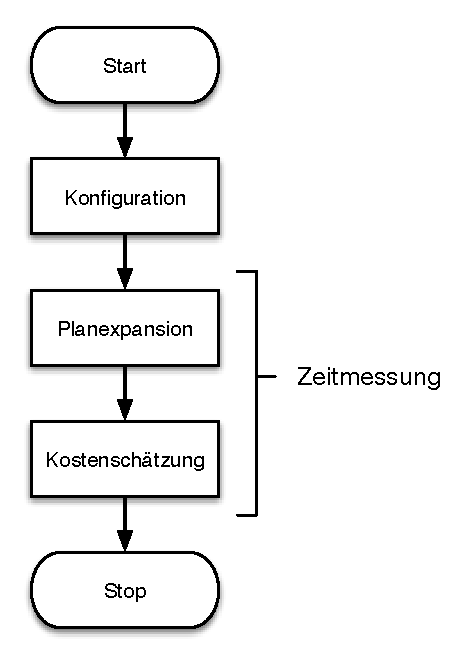
\includegraphics[scale=0.8]{04_Implementierung/00_media/Ablauf.pdf}
  \caption{Ablauf der eigenen Implementierung}
  \label{Ablauf}
\end{figure}

Die Ausführung des Programms geschieht in drei Schritten (vgl. Abb. \ref{Ablauf}): (1) Konfiguration, (2) Generierung von semantisch gleichen Plänen, (3) Finden des optimalen Plans.




Im ersten Schritt, wird auf Grund von externen Parametern das System konfiguriert. Die Konfiguration erfolgt durch ein JSON File. In ihm werden die Parameter (Relationen und deren Kardinalität, Join-Kanten und deren Selektivität, initialer Plan und Regelmengen) für die Optimierung festgelegt. Mit Hilfe der Relationen und deren Kardinalität können später im Zusammenspiel mit Join-Kanten und Selektivität die Kosten für einen Plan berechnet werden. Der initiale Plan dient als Startpunkt der Transformation. Auf ihn werden die Regelmengen angewendet und so logische  Äquivalente erzeugt.

Zu Beginn des zweiten Schritts, der Erzeugung von äquivalenten Plänen, wird die Zeitmessung gestartet.  Mit Hilfe von Enumeratoren werden die unterschiedlichen Regelmengen auf den initialen Plan angewendet.

In einem finalen Schritt findet die Kostenberechnung statt um aus den möglichen Plänen den günstigsten auszuwählen. Diese Preisberechnung wird im Modul der Kostenschätzung vollzogen.



\begin{figure}[ht]
  \centering
  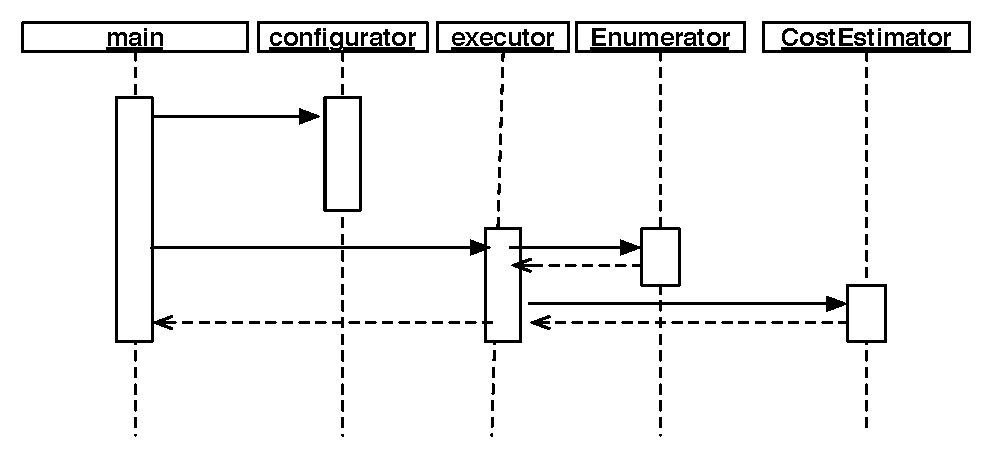
\includegraphics[width=\textwidth]{04_Implementierung/00_media/SequenceDiagramConfiguration.pdf}
  \caption{Sequenzdiagramm: Aufruf der einzelnen Komponenten}
  \label{SequenceDiagramConfiguration}
\end{figure}


Der genaue Ablauf des Programms lässt sich in Abbildung \ref{SequenceDiagramConfiguration} ablesen. Das Sequenzdiagram beginnt mit der Hauptmethode. Diese Hauptmethode erhält durch den Konfigurator die aktuelle Konfiguration. Einer Executor genannten Klasse wird diese Konfiguration übergeben. Der Executer stellt den Test zusammen, wählt den Enumerator und die Regelmenge aus. Die Zeitmessung wird gestartet und aus ein initaler Plan an den Enumerator übergeben. Sobald die Enumeration abgeschlossen ist, beginnt die Kostenschätzung. Nach Abschluss der Kostenschätzung wird die Zeitmessung angehalten. Je nachdem ob weitere Test-Szenarien vorgesehen sind wird der Executor erneut aufgerufen. Andernfalls ist an dieser Stelle das Programm beendet und die Messung kann an den Nutzer ausgegeben werden.
